\documentclass[aspectratio=169]{beamer}

\usetheme{Boadilla}
\usefonttheme{professionalfonts}
\setbeamertemplate{navigation symbols}{}
\setbeamertemplate{itemize items}[circle]
\setbeamertemplate{enumerate items}[default]
\setbeamertemplate{headline}{}

\usepackage[utf8]{inputenc}
\usepackage[T1]{fontenc}
\usepackage{lmodern}
\usepackage{amsmath}
\usepackage{booktabs}
\usepackage{tabularx}
\usepackage{array}
\usepackage{hyperref}
\usepackage[strings]{underscore}
\usepackage{listings}
\usepackage{tikz}
\usetikzlibrary{arrows.meta,positioning,fit,calc,shapes.geometric}
\usepackage{xcolor}

\definecolor{courseblue}{HTML}{12355B}
\definecolor{coursegold}{HTML}{C98A2E}
\definecolor{courseice}{HTML}{EEF3F8}
\definecolor{coursegreen}{HTML}{2F6B4F}
\definecolor{coursegray}{HTML}{4B5563}
\definecolor{codebg}{HTML}{F7F9FC}
\definecolor{codecomment}{HTML}{5E6C84}
\definecolor{codestring}{HTML}{0B6E4F}

\setbeamercolor{palette primary}{bg=courseblue,fg=white}
\setbeamercolor{palette secondary}{bg=coursegold,fg=white}
\setbeamercolor{palette tertiary}{bg=courseblue,fg=white}
\setbeamercolor{palette quaternary}{bg=coursegold,fg=white}
\setbeamercolor{structure}{fg=courseblue}
\setbeamercolor{frametitle}{bg=courseice,fg=courseblue}
\setbeamercolor{title}{fg=courseblue}
\setbeamercolor{block title}{bg=courseblue,fg=white}
\setbeamercolor{block body}{bg=courseice,fg=black}
\setbeamercolor{normal text}{fg=black,bg=white}
\setbeamercolor{alerted text}{fg=coursegold}

\setbeamerfont{footline}{size=\scriptsize}

\setbeamertemplate{footline}{
  \leavevmode
  \hbox{
    \begin{beamercolorbox}[wd=.33\paperwidth,ht=2.8ex,dp=1.2ex,leftskip=0.8em]{palette primary}%
      University of Trieste
    \end{beamercolorbox}%
    \begin{beamercolorbox}[wd=.49\paperwidth,ht=2.8ex,dp=1.2ex,center]{palette tertiary}%
      \coursename{} \textbar{} \coursecode
    \end{beamercolorbox}%
    \begin{beamercolorbox}[wd=.18\paperwidth,ht=2.8ex,dp=1.2ex,rightskip=0.8em plus1fil]{palette secondary}%
      \insertframenumber{} / \inserttotalframenumber
    \end{beamercolorbox}%
  }
}

\hypersetup{
  colorlinks=true,
  linkcolor=courseblue,
  urlcolor=coursegreen
}

\lstdefinestyle{coursepython}{
  language=Python,
  basicstyle=\ttfamily\footnotesize,
  keywordstyle=\color{courseblue}\bfseries,
  commentstyle=\color{codecomment}\itshape,
  stringstyle=\color{codestring},
  showstringspaces=false,
  columns=fullflexible,
  keepspaces=true,
  frame=single,
  framerule=0.6pt,
  rulecolor=\color{courseblue},
  backgroundcolor=\color{codebg},
  xleftmargin=0.4em,
  xrightmargin=0.4em,
  aboveskip=0.4em,
  belowskip=0.2em
}

\newcommand{\coursename}{Data-driven Systems Engineering}
\newcommand{\coursecode}{440MI / 305SM}
\newcommand{\coursefooter}{}

\newcommand{\learninggoals}[1]{
  \begin{block}{Learning goals}
  #1
  \end{block}
}

\newcommand{\repoactivity}[1]{
  \begin{block}{Repo activity}
  #1
  \end{block}
}

\newcommand{\readinglist}[1]{
  \begin{block}{Papers and materials}
  {\footnotesize #1}
  \end{block}
}

\newcommand{\coursecontextframe}[5]{
  \begin{frame}{Course Map and Running Cases}
  \centering
  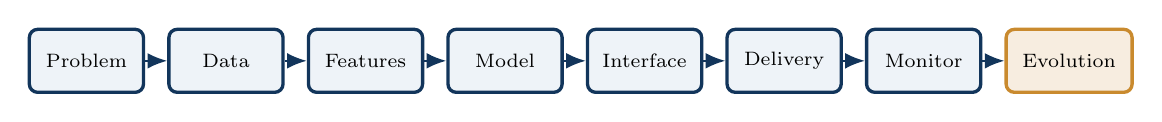
\begin{tikzpicture}[node distance=0.28cm]
  \node[flowbox, minimum width=1.45cm, minimum height=0.8cm] (problem) {\scriptsize Problem};
  \node[flowbox, minimum width=1.45cm, minimum height=0.8cm, right=of problem] (data) {\scriptsize Data};
  \node[flowbox, minimum width=1.45cm, minimum height=0.8cm, right=of data] (features) {\scriptsize Features};
  \node[flowbox, minimum width=1.45cm, minimum height=0.8cm, right=of features] (model) {\scriptsize Model};
  \node[flowbox, minimum width=1.45cm, minimum height=0.8cm, right=of model] (interface) {\scriptsize Interface};
  \node[flowbox, minimum width=1.45cm, minimum height=0.8cm, right=of interface] (delivery) {\scriptsize Delivery};
  \node[flowbox, minimum width=1.45cm, minimum height=0.8cm, right=of delivery] (monitor) {\scriptsize Monitor};
  \node[accentbox, minimum width=1.6cm, minimum height=0.8cm, right=of monitor] (evolution) {\scriptsize Evolution};
  \foreach \a/\b in {problem/data,data/features,features/model,model/interface,interface/delivery,delivery/monitor,monitor/evolution} {
    \draw[arrow] (\a) -- (\b);
  }
  \end{tikzpicture}

  \vspace{0.5em}
  \begin{block}{Today in the course}
  \textbf{Focus:} #1

  \textbf{Bridge:} #2
  \end{block}

  \begin{columns}[T]
  \column{0.48\textwidth}
  \begin{block}{Fraud case}
  {\footnotesize #3}
  \end{block}
  \column{0.48\textwidth}
  \begin{block}{Pasteurization case}
  {\footnotesize #4}
  \end{block}
  \end{columns}

  \vspace{0.3em}
  {\footnotesize \textbf{Course thread:} #5}
  \coursefooter
  \end{frame}
}

\newcommand{\classclosingframe}[4]{
  \begin{frame}{From This Class to the Next}
  \begin{block}{What stays with us}
  #1
  \end{block}

  \begin{columns}[T]
  \column{0.48\textwidth}
  \begin{block}{Project use}
  {\footnotesize #2}
  \end{block}
  \column{0.48\textwidth}
  \begin{block}{Next connection}
  {\footnotesize #3}
  \end{block}
  \end{columns}

  \vspace{0.3em}
  {\footnotesize \textbf{Course thread:} #4}
  \coursefooter
  \end{frame}
}

\tikzset{
  flowbox/.style={
    rounded corners=3pt,
    draw=courseblue,
    fill=courseice,
    very thick,
    minimum width=2.2cm,
    minimum height=0.9cm,
    align=center,
    font=\small
  },
  accentbox/.style={
    rounded corners=3pt,
    draw=coursegold,
    fill=coursegold!15,
    very thick,
    minimum width=2.2cm,
    minimum height=0.9cm,
    align=center,
    font=\small
  },
  arrow/.style={
    -{Latex[length=2.5mm,width=2mm]},
    thick,
    draw=courseblue
  }
}


\title{Class 11: Software Process Models}
\author{\coursename}
\date{}

\begin{document}

\frame{\titlepage \coursefooter}

\begin{frame}{Agenda}
\begin{itemize}
\item Why process models exist and what they control
\item Process descriptions and the four core activities
\item Plan-driven, incremental, and hybrid approaches
\item Waterfall versus agile in software and ML work
\item Agile history, manifesto, principles, and drawbacks
\item Process selection for ML-enabled systems
\end{itemize}
\coursefooter
\end{frame}

\begin{frame}{Process models are decision tools}
\learninggoals{
\begin{itemize}
\item Compare plan-driven, incremental, and hybrid approaches.
\item Understand why ML projects often need hybrid processes.
\item Match process choice to uncertainty, regulation, and team maturity.
\item Explain how process decisions affect documentation, testing, and release risk.
\end{itemize}
}
\coursefooter
\end{frame}

\coursecontextframe
{Choosing a development process that fits uncertainty and risk.}
{This class bridges from requirements into delivery strategy by asking how teams should organize work across exploration, validation, and release.}
{In the fraud case, agile iteration helps with thresholds and features, while controlled release gates protect the production path.}
{In the pasteurization case, exploratory modeling may be agile, but operational deployment benefits from stronger validation and change control.}
{The course thread is that process choice shapes how every later activity gets coordinated.}

\begin{frame}{Why software teams need process models}
\begin{itemize}
\item A process model makes coordination explicit: who decides, who reviews, and what evidence is required.
\item It reduces confusion around sequencing, approvals, and handoffs.
\item It creates a shared language for planning, validation, and improvement.
\item In ML systems, it also helps separate exploratory work from production commitments.
\end{itemize}
\begin{block}{Key idea}
Process is not bureaucracy by definition. A good process reduces friction by clarifying how work moves from idea to dependable outcome.
\end{block}
\coursefooter
\end{frame}

\begin{frame}{Process descriptions}
\begin{itemize}
\item Activities: for example data modeling, UI design, service integration.
\item Products: documents, code, models, dashboards, tests.
\item Roles: analyst, developer, data scientist, reviewer, operator.
\item Pre- and post-conditions: what must be true before and after an activity.
\end{itemize}
\coursefooter
\end{frame}

\begin{frame}{The four core process activities}
\begin{columns}[T]
\column{0.48\textwidth}
\begin{itemize}
\item Specification
\item Development
\item Validation
\item Evolution
\end{itemize}
\column{0.48\textwidth}
\begin{itemize}
\item Define the problem and constraints.
\item Build software, data pipelines, and models.
\item Check quality, fit, and safety.
\item Adapt after feedback, incidents, and change.
\end{itemize}
\end{columns}
\vspace{0.5em}
\begin{block}{ML-specific nuance}
Evolution includes code change, data change, feature change, threshold change, and sometimes retraining under new operating conditions.
\end{block}
\coursefooter
\end{frame}

\begin{frame}{Waterfall, agile, and hybrid in one view}
\begin{tabularx}{\textwidth}{>{\bfseries}l X X}
Model & Strength & Main risk \\
\toprule
Waterfall & Strong control and documentation & Adapts poorly to late discoveries \\
Agile & Fast feedback and iteration & Can drift without disciplined scope control \\
Hybrid & Exploration plus governance & Needs explicit handoff rules \\
\bottomrule
\end{tabularx}
\coursefooter
\end{frame}

\begin{frame}{Plan-driven processes}
\begin{itemize}
\item Activities are planned in advance and progress is measured against the plan.
\item Works well when scope is stable, interfaces are fixed, and coordination cost is high.
\item Documentation and formal review are first-class artifacts, not afterthoughts.
\item Best fit often appears in safety-critical, regulated, or externally audited systems.
\end{itemize}
\begin{block}{Example}
Healthcare decision support, industrial control, or finance platforms may need strong traceability before release.
\end{block}
\coursefooter
\end{frame}

\begin{frame}{Incremental and agile processes}
\begin{itemize}
\item Work is delivered in usable increments so learning can happen early.
\item Specification, design, and implementation become interleaved.
\item Customer feedback changes priorities continuously.
\item Small releases reduce the cost of being wrong, but only if the team keeps a strong definition of done.
\end{itemize}
\coursefooter
\end{frame}

\begin{frame}{Waterfall versus agile in this course}
\begin{columns}[T]
\column{0.48\textwidth}
\textbf{Waterfall strengths}
\begin{itemize}
\item Stable scope
\item Formal sign-off
\item Easier external audit
\end{itemize}
\column{0.48\textwidth}
\textbf{Agile strengths}
\begin{itemize}
\item Fast feedback
\item Iterative learning
\item Better fit for uncertain data work
\end{itemize}
\end{columns}
\coursefooter
\end{frame}

\begin{frame}{Incremental delivery reduces downtime risk}
\begin{itemize}
\item In a monolithic release, many changes arrive at once and rollback becomes expensive.
\item In incremental delivery, small changes can be isolated, tested, and reverted more safely.
\item This is one reason CI/CD and agile practices complement each other.
\end{itemize}
\begin{block}{Example}
An e-commerce platform can deploy login first, then cart, then payment. A fraud API can deploy logging, then scoring, then alert routing instead of changing everything at once.
\end{block}
\coursefooter
\end{frame}

\begin{frame}{Why ML work often needs hybrid delivery}
\begin{itemize}
\item Early phases are exploratory: data quality, labels, and metrics are uncertain.
\item Later phases need discipline: deployment, interfaces, testing, and compliance.
\item Regulated contexts cannot rely on verbal agreements or informal notebooks.
\end{itemize}
\begin{block}{Example}
An industrial monitoring system may use agile prototyping for the predictor, then a more controlled process for deployment in the plant network.
\end{block}
\coursefooter
\end{frame}

\begin{frame}{A hybrid lifecycle for data-driven systems}
\centering
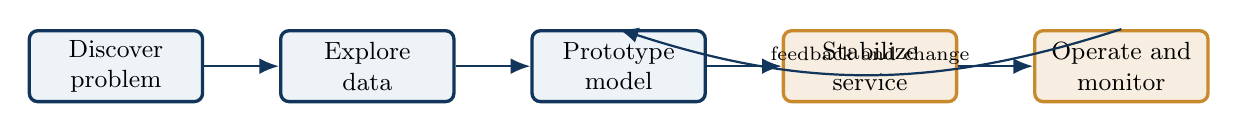
\begin{tikzpicture}[node distance=0.85cm and 0.95cm]
\node[flowbox] (discover) {Discover\\problem};
\node[flowbox, right=of discover] (explore) {Explore\\data};
\node[flowbox, right=of explore] (prototype) {Prototype\\model};
\node[accentbox, right=of prototype] (stabilize) {Stabilize\\service};
\node[accentbox, right=of stabilize] (operate) {Operate and\\monitor};
\draw[arrow] (discover) -- (explore);
\draw[arrow] (explore) -- (prototype);
\draw[arrow] (prototype) -- (stabilize);
\draw[arrow] (stabilize) -- (operate);
\draw[arrow, bend left=18] (operate.north) to node[above, font=\scriptsize] {feedback and change} (prototype.north);
\end{tikzpicture}
\vspace{0.5em}
\begin{itemize}
\item The point of a hybrid process is matching control to uncertainty.
\end{itemize}
\coursefooter
\end{frame}

\begin{frame}{Useful classroom comparison}
\begin{columns}[T]
\column{0.5\textwidth}
\textbf{Fraud API project}
\begin{itemize}
\item Agile for feature and threshold iteration
\item Structured release gates
\item Monitoring after deployment
\end{itemize}
\column{0.5\textwidth}
\textbf{Hospital ML support tool}
\begin{itemize}
\item Stronger requirement control
\item Formal validation and logging
\item Slower but safer release cadence
\end{itemize}
\end{columns}
\coursefooter
\end{frame}

\begin{frame}{Why agile emerged}
\begin{itemize}
\item Agile methods grew partly from dissatisfaction with heavyweight software methods in the 1980s and 1990s.
\item Teams wanted faster delivery, lower overhead, and better response to changing requirements.
\item The emphasis shifted from exhaustive up-front design toward working software and rapid learning.
\end{itemize}
\begin{block}{Important caution}
Agile was never meant to mean ``no design'' or ``no documentation.'' It means documentation and planning should earn their cost.
\end{block}
\coursefooter
\end{frame}

\begin{frame}{Agile manifesto and principles}
\begin{itemize}
\item Individuals and interactions over processes and tools.
\item Working software over comprehensive documentation.
\item Customer collaboration over contract negotiation.
\item Responding to change over following a plan.
\end{itemize}
\begin{block}{Important nuance}
The right side still matters. In ML projects, documentation, governance, and change control return quickly once deployment begins.
\end{block}
\coursefooter
\end{frame}

\begin{frame}{Agile principles adapted to ML teams}
\begin{itemize}
\item Customer involvement: stakeholders help define value and review increments.
\item Incremental delivery: baselines, APIs, dashboards, and monitoring can each be delivered in stages.
\item People over process: expertise matters when requirements and data are still uncertain.
\item Embrace change: feedback from errors, labels, or operations is expected.
\item Maintain simplicity: avoid unnecessary features, pipelines, and tools.
\end{itemize}
\coursefooter
\end{frame}

\begin{frame}{Drawbacks and failure modes}
\begin{itemize}
\item Customers may disengage from the constant feedback cycle.
\item Multiple stakeholders may prioritize conflicting changes.
\item Teams can confuse speed with lack of discipline.
\item Without clear definitions of done, iteration turns into churn.
\end{itemize}
\coursefooter
\end{frame}

\begin{frame}{How to choose a process model}
\begin{tabularx}{\textwidth}{>{\bfseries}l X}
Question & Process implication \\
\toprule
Are requirements stable? & More stability supports plan-driven structure. \\
Is data quality uncertain? & More uncertainty favors iterative exploration. \\
Is the system regulated? & More regulation requires stronger documentation and approval. \\
Are releases frequent? & Frequent change favors incremental delivery and automation. \\
Will the model evolve in production? & Evolution demands monitoring and change governance. \\
\bottomrule
\end{tabularx}
\coursefooter
\end{frame}

\begin{frame}{What students should defend in presentations}
\begin{itemize}
\item Why they chose their process.
\item Where requirements may still change.
\item Which artifacts create team alignment.
\item When they move from experimentation to controlled delivery.
\end{itemize}
\coursefooter
\end{frame}

\classclosingframe
{\begin{itemize}
\item No process model is universally best; the fit depends on uncertainty, feedback speed, and governance needs.
\item ML projects often need iterative discovery without losing engineering control.
\item Process choice affects documentation, coordination, testing, and release rhythm.
\end{itemize}}
{Project teams should now be able to justify whether their work needs more exploratory loops, more structure, or a hybrid approach.}
{Class 12 narrows that process discussion into practical agile tools such as backlogs, stories, boards, ceremonies, and feedback loops.}
{After selecting a development posture, we translate it into everyday coordination practices the team can actually run.}

\begin{frame}{Papers and materials}
\readinglist{
\href{https://agilemanifesto.org/}{Agile Manifesto};\ 
\href{https://www.pearson.com/en-us/subject-catalog/p/software-engineering/P200000003144/9780137035151}{Sommerville, Software Engineering};\ 
\href{https://martinfowler.com/articles/newMethodology.html}{Martin Fowler on the new methodology};\ 
\href{https://www.scrumguides.org/}{The Scrum Guide};\ 
\href{https://queue.acm.org/detail.cfm?id=3454124}{Production AI lifecycle discussion in ACM Queue}.
}
\coursefooter
\end{frame}

\end{document}
